\label{md__devices_Devices}%
\hypertarget{md__devices_Devices}{}%


Devices are the entities that allow {\itshape faudio} to communicate with the outside world. Any client will need to connect at least two devices to each other to form a audio stream. While signals and processors denote functions, devices denote sources and sinks of audio data, such as files, memory buffers or audio hardware.

Devices are grouped into {\itshape real-\/time devices}, {\itshape non-\/real-\/time devices}. Audio and midi information are handled by different devices. Note that {\itshape faudio} does not provide non-\/real-\/time midi at the moment\-: if you need to parse and process a midi file you must use some other method.\hypertarget{md__devices_RealTime}{}\section{Real time devices}\label{md__devices_RealTime}
\hypertarget{md__devices_SessionsAndStreams}{}\subsection{Sessions and streams}\label{md__devices_SessionsAndStreams}
{\itshape faudio} provides access to real-\/time devices through of {\itshape sessions}, and {\itshape streams}. While a {\itshape device} provides access to an external audio interface, a {\itshape session} provides access to the entire audio system, and a {\itshape stream} to a specific audio computation. These concepts are hierarchical, each stream is associated with a device and each device with a session.

Typically, each physical audio or midi interface is represented by a single device in {\itshape faudio}. The operating system may also provide abstract devices, representing network connections, software mixers and the like.

{\itshape faudio} places certain restrictions on the order or acquisition of sessions, devices and streams. Any client that wants to obtain a device must first initiate a session. The initialization of a session may fail, for example if the underlying audio system is already being used by an exclusive process. If it succeeds, a handle to the underlying session is provided. This handle allow the user to inspect the set of devices available in the sesssion. The client may then open a stream.

T\-O\-D\-O


\begin{DoxyImage}
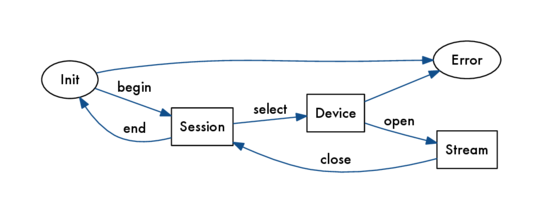
\includegraphics[width=0.8\textwidth]{device_states}
\caption{State transactions of the audio system (simplified)}
\end{DoxyImage}


\begin{DoxyNote}{Note}
The semantics of {\itshape streams} have been changed from earlier versions of {\itshape faudio}, in which a {\itshape stream} could be repeatedly stopped and started.
\end{DoxyNote}
\hypertarget{md__devices_Notifications}{}\subsection{Session notifications}\label{md__devices_Notifications}
Sessions represent a snapshot of the setup at the time it was initiated; the set of available devices in a specific session will never change. If a change in the underlying audio system is detected while a session is still active, a new session has to be started to observe the new setup.

You can register a callback to be invoked when the a possible change in hardware setup is detected, see fa\-\_\-\-\_\-audio\-\_\-set\-\_\-status\-\_\-callback. Note that this callback may be invoked in an interrupt handler thread and that the task of ending a session should generally be handled in the same thread that created the session. Use an atomic reference or a condition variable to communicate the notification to the appropriate thread.\hypertarget{md__devices_AudioStreams}{}\subsection{Audio streams}\label{md__devices_AudioStreams}
\hypertarget{md__devices_AudioAR}{}\subsubsection{Imperative style}\label{md__devices_AudioAR}
The acquire-\/release style use a paired method pattern. You call a creation method to get a value, and a destruction method to release. Note that devices, sessions and streams have single-\/ownership semantics.


\begin{DoxyCode}
\textcolor{preprocessor}{#include <\hyperlink{fa_2fa_8h}{fa/fa.h}>}

\textcolor{keywordtype}{int} main (\textcolor{keywordtype}{int} argc, \textcolor{keywordtype}{char} \textcolor{keyword}{const} *argv[])
\{
    \hyperlink{group___fa_audio_session_ga62ee22268c23f1b18447141feccc01e0}{fa\_audio\_session\_t}     session;
    \hyperlink{group___fa_audio_device_ga03de89ee66c6465f8cedd3a0286598f4}{fa\_audio\_device\_t}      input, output;
    \hyperlink{group___fa_audio_stream_ga78fbee3026130ce00d8e00a4e73a84c3}{fa\_audio\_stream\_t}      stream
    \hyperlink{group___fa_signal_gac5c72f160cd6e93a6783551627b166e5}{fa\_signal\_t}            id;

    \textcolor{comment}{// Processor to use}
    \textcolor{keywordtype}{id} = fa\_signal\_identity();

    \textcolor{comment}{// Begin session}
    session = \hyperlink{group___fa_audio_session_ga0022e6e72ee2f2c4c04a6165847a50dd}{fa\_audio\_begin\_session}();
    \textcolor{keywordflow}{if} (\hyperlink{group___fa_gaec61e23c174faf5e5244ae876d264eb5}{fa\_check}(stream)) \{
        \hyperlink{group___fa_error_ga466e0539bedb29f68527448ed9ba11bf}{fa\_error\_log}(stream);
        \textcolor{keywordflow}{goto} cleanup;

    \} \textcolor{keywordflow}{else} \{
        \textcolor{comment}{// Session obtained, we can now access devices}
        input  = \hyperlink{group___fa_audio_device_ga690374b4ffcee314cb4cdad6309ef817}{fa\_audio\_default\_input}(session);
        input  = \hyperlink{group___fa_audio_device_ga364583565c9405e541ae52e41efa38e7}{fa\_audio\_default\_output}(session);

        \textcolor{comment}{// Start stream}
        stream = \hyperlink{group___fa_audio_stream_ga912f03969d6207dd40a2746e62888adb}{fa\_audio\_open\_stream}(input, \textcolor{keywordtype}{id}, output);
        \textcolor{keywordflow}{if} (\hyperlink{group___fa_gaec61e23c174faf5e5244ae876d264eb5}{fa\_check}(stream)) \{
            \hyperlink{group___fa_error_ga466e0539bedb29f68527448ed9ba11bf}{fa\_error\_log}(stream);
            \textcolor{keywordflow}{goto} cleanup;

        \} \textcolor{keywordflow}{else} \{
            \textcolor{comment}{// Stream active, let it run for 5 seconds}
            \hyperlink{group___fa_thread_ga6a6c70317be48603d0316bdb93914f5f}{fa\_thread\_sleep}(5000);
        \}
    \}

    \textcolor{comment}{// Cleanup}
cleanup:
    \hyperlink{group___fa_ga6fd6818b190b9e41a3b5f07e78638539}{fa\_destroy}(stream);
    \hyperlink{group___fa_ga6fd6818b190b9e41a3b5f07e78638539}{fa\_destroy}(session);
    \hyperlink{group___fa_ga6fd6818b190b9e41a3b5f07e78638539}{fa\_destroy}(\textcolor{keywordtype}{id});
\}
\end{DoxyCode}
\hypertarget{md__devices_AudioCB}{}\subsubsection{Callback style}\label{md__devices_AudioCB}
The callback style require that you provide a callback to be invoked when the session or stream is valid. Destruction is handled automatically after this method has returned. Errors are handled by a special callback, to which you can pass \hyperlink{group___fa_error_ga466e0539bedb29f68527448ed9ba11bf}{fa\-\_\-error\-\_\-log}, or a user defined function.


\begin{DoxyCode}
\textcolor{preprocessor}{#include <\hyperlink{fa_2fa_8h}{fa/fa.h}>}
\textcolor{preprocessor}{#include <\hyperlink{util_8h}{fa/util.h}>}

stream\_t run\_callback(stream\_t stream)
\{
    \textcolor{comment}{// Stream active, let it run for 5 seconds}
    \hyperlink{group___fa_thread_ga6a6c70317be48603d0316bdb93914f5f}{fa\_thread\_sleep}(\hyperlink{util_8h_a1a3cd4cff330c981ed89bbd3a3426273}{seconds}(10));
    \textcolor{keywordflow}{return} stream;
\}

session\_t session\_callback(\textcolor{keywordtype}{void}* data, session\_t session)
\{
    \hyperlink{group___fa_audio_device_ga03de89ee66c6465f8cedd3a0286598f4}{fa\_audio\_device\_t}    input, output;
    \hyperlink{group___fa_signal_gac5c72f160cd6e93a6783551627b166e5}{fa\_signal\_t}          id;

    \textcolor{comment}{// Session obtained, we can now access devices}
    input   = \hyperlink{group___fa_audio_device_ga690374b4ffcee314cb4cdad6309ef817}{fa\_audio\_default\_input}(session);
    output  = \hyperlink{group___fa_audio_device_ga690374b4ffcee314cb4cdad6309ef817}{fa\_audio\_default\_input}(session);
    \textcolor{keywordtype}{id}      = (signal\_t*) data;

    \textcolor{comment}{// Start stream}
    \hyperlink{group___fa_audio_stream_gaa385a92b31401915477027e03a39094e}{fa\_audio\_with\_stream}(input, \textcolor{keywordtype}{id}, output,
                          run\_callback, \hyperlink{group___fa_error_ga466e0539bedb29f68527448ed9ba11bf}{fa\_error\_log}, NULL);

    \hyperlink{group___fa_ga6fd6818b190b9e41a3b5f07e78638539}{fa\_destroy}(\textcolor{keywordtype}{id});
    \textcolor{keywordflow}{return} session;
\}

\textcolor{keywordtype}{int} main (\textcolor{keywordtype}{int} argc, \textcolor{keywordtype}{char} \textcolor{keyword}{const} *argv[])
\{                  
    \textcolor{comment}{// Processor to use}
    \hyperlink{group___fa_signal_gac5c72f160cd6e93a6783551627b166e5}{fa\_signal\_t} signal = fa\_signal\_identity();

    \textcolor{comment}{// Begin session}
    \hyperlink{group___fa_audio_session_gabbec6678e24f6476ac04f7d759ec7ffb}{fa\_audio\_with\_session}(session\_callback, \textcolor{keywordtype}{id},
                           \hyperlink{group___fa_error_ga466e0539bedb29f68527448ed9ba11bf}{fa\_error\_log}, NULL);
\}
\end{DoxyCode}
\hypertarget{md__devices_id8127832}{}\section{Non-\/realtime devices}\label{md__devices_id8127832}
\hypertarget{md__devices_id98281723}{}\subsection{The run method}\label{md__devices_id98281723}
T\-O\-D\-O\hypertarget{md__devices_id9192746}{}\subsection{File devices}\label{md__devices_id9192746}

\begin{DoxyCode}
\textcolor{preprocessor}{#include <\hyperlink{fa_2fa_8h}{fa/fa.h}>}

\textcolor{keyword}{typedef} fa\_file\_t      device\_t;
\textcolor{keyword}{typedef} \hyperlink{group___fa_signal_gac5c72f160cd6e93a6783551627b166e5}{fa\_signal\_t}    \hyperlink{util_8h_a4179e0566b0727e21f1fd4b5e6533dee}{signal\_t};

\textcolor{keywordtype}{int} main (\textcolor{keywordtype}{int} argc, \textcolor{keywordtype}{char} \textcolor{keyword}{const} *argv[])
\{
    fa\_device\_t    input, output;
    \hyperlink{group___fa_signal_gac5c72f160cd6e93a6783551627b166e5}{fa\_signal\_t}    id;
    fa\_result\_t    result;

    \textcolor{comment}{// Processor to use}
    \textcolor{keywordtype}{id} = fa\_signal\_identity();

    \textcolor{comment}{// Open streams}
    input   = fa\_\_file\_open(\textcolor{keywordtype}{string}(\textcolor{stringliteral}{"test/in.wav"}));
    output  = fa\_\_file\_open(\textcolor{keywordtype}{string}(\textcolor{stringliteral}{"test/out.wav"}));

    \textcolor{comment}{// Handle possible errors}
    \textcolor{keywordflow}{if} (\hyperlink{group___fa_gaec61e23c174faf5e5244ae876d264eb5}{fa\_check}(input)) \{
        \hyperlink{group___fa_error_ga466e0539bedb29f68527448ed9ba11bf}{fa\_error\_log}(result);
    \}                                    

    \textcolor{keywordflow}{if} (\hyperlink{group___fa_gaec61e23c174faf5e5244ae876d264eb5}{fa\_check}(output)) \{
        \hyperlink{group___fa_error_ga466e0539bedb29f68527448ed9ba11bf}{fa\_error\_log}(result);
    \}                                    

    result  = fa\_\_file\_run(in, \textcolor{keywordtype}{id}, out);

    \textcolor{comment}{// Handle possible error}
    \textcolor{keywordflow}{if} (\hyperlink{group___fa_gaec61e23c174faf5e5244ae876d264eb5}{fa\_check}(result)) \{
        \hyperlink{group___fa_error_ga466e0539bedb29f68527448ed9ba11bf}{fa\_error\_log}(result);
    \}                                    

    \hyperlink{group___fa_ga6fd6818b190b9e41a3b5f07e78638539}{fa\_destroy}(input);
    \hyperlink{group___fa_ga6fd6818b190b9e41a3b5f07e78638539}{fa\_destroy}(output);;
\}
\end{DoxyCode}
\hypertarget{md__devices_id11127283}{}\subsection{Buffer devices}\label{md__devices_id11127283}

\begin{DoxyCode}
\textcolor{preprocessor}{#include <\hyperlink{fa_2fa_8h}{fa/fa.h}>}

\textcolor{keyword}{typedef} fa\_file\_t   device\_t;
\textcolor{keyword}{typedef} \hyperlink{group___fa_signal_gac5c72f160cd6e93a6783551627b166e5}{fa\_signal\_t} \hyperlink{util_8h_a4179e0566b0727e21f1fd4b5e6533dee}{signal\_t};

\textcolor{keywordtype}{int} main (\textcolor{keywordtype}{int} argc, \textcolor{keywordtype}{char} \textcolor{keyword}{const} *argv[])
\{
    device\_t    input, output;
    signal\_t    id;
    result\_t    result;

    \textcolor{comment}{// Processor to use}
    \textcolor{keywordtype}{id} = fa\_signal\_identity();

    \textcolor{comment}{// Open streams}
    input   = fa\_buffer\_open(\hyperlink{group___fa_buffer_ga67c4124d193bca81a6e21ec04d9ff832}{fa\_buffer\_create}(1024));
    output  = fa\_buffer\_open(\hyperlink{group___fa_buffer_ga67c4124d193bca81a6e21ec04d9ff832}{fa\_buffer\_create}(1024));

    \textcolor{comment}{// Handle possible errors}
    \textcolor{keywordflow}{if} (\hyperlink{group___fa_gaec61e23c174faf5e5244ae876d264eb5}{fa\_check}(input)) \{
        \hyperlink{group___fa_error_ga466e0539bedb29f68527448ed9ba11bf}{fa\_error\_log}(result);
    \}                                    

    \textcolor{keywordflow}{if} (\hyperlink{group___fa_gaec61e23c174faf5e5244ae876d264eb5}{fa\_check}(output)) \{
        \hyperlink{group___fa_error_ga466e0539bedb29f68527448ed9ba11bf}{fa\_error\_log}(result);
    \}                                    

    result  = fa\_buffer\_run(in, \textcolor{keywordtype}{id}, out);

    \textcolor{comment}{// Handle possible error}
    \textcolor{keywordflow}{if} (\hyperlink{group___fa_gaec61e23c174faf5e5244ae876d264eb5}{fa\_check}(result)) \{
        \hyperlink{group___fa_error_ga466e0539bedb29f68527448ed9ba11bf}{fa\_error\_log}(result);
    \}                                    

    \hyperlink{group___fa_ga6fd6818b190b9e41a3b5f07e78638539}{fa\_destroy}(input);
    \hyperlink{group___fa_ga6fd6818b190b9e41a3b5f07e78638539}{fa\_destroy}(output);
\}
\end{DoxyCode}
 